\section{Operating Basics}

\subsection{Introduction}

To ensure a good understanding of controllers and controlling theory, a laboratory experiment was performed. As the plant, a motor was used whose speed had to be controlled.
The step function was measured and analyzed at first. Knowing the step function it was very easy to implement a suitable PID controller.

\subsection{Step Function}

To determine the characteristics of the system, a step is applied to the input. Then the output is observed.

\begin{figure}[H]
\begin{center}
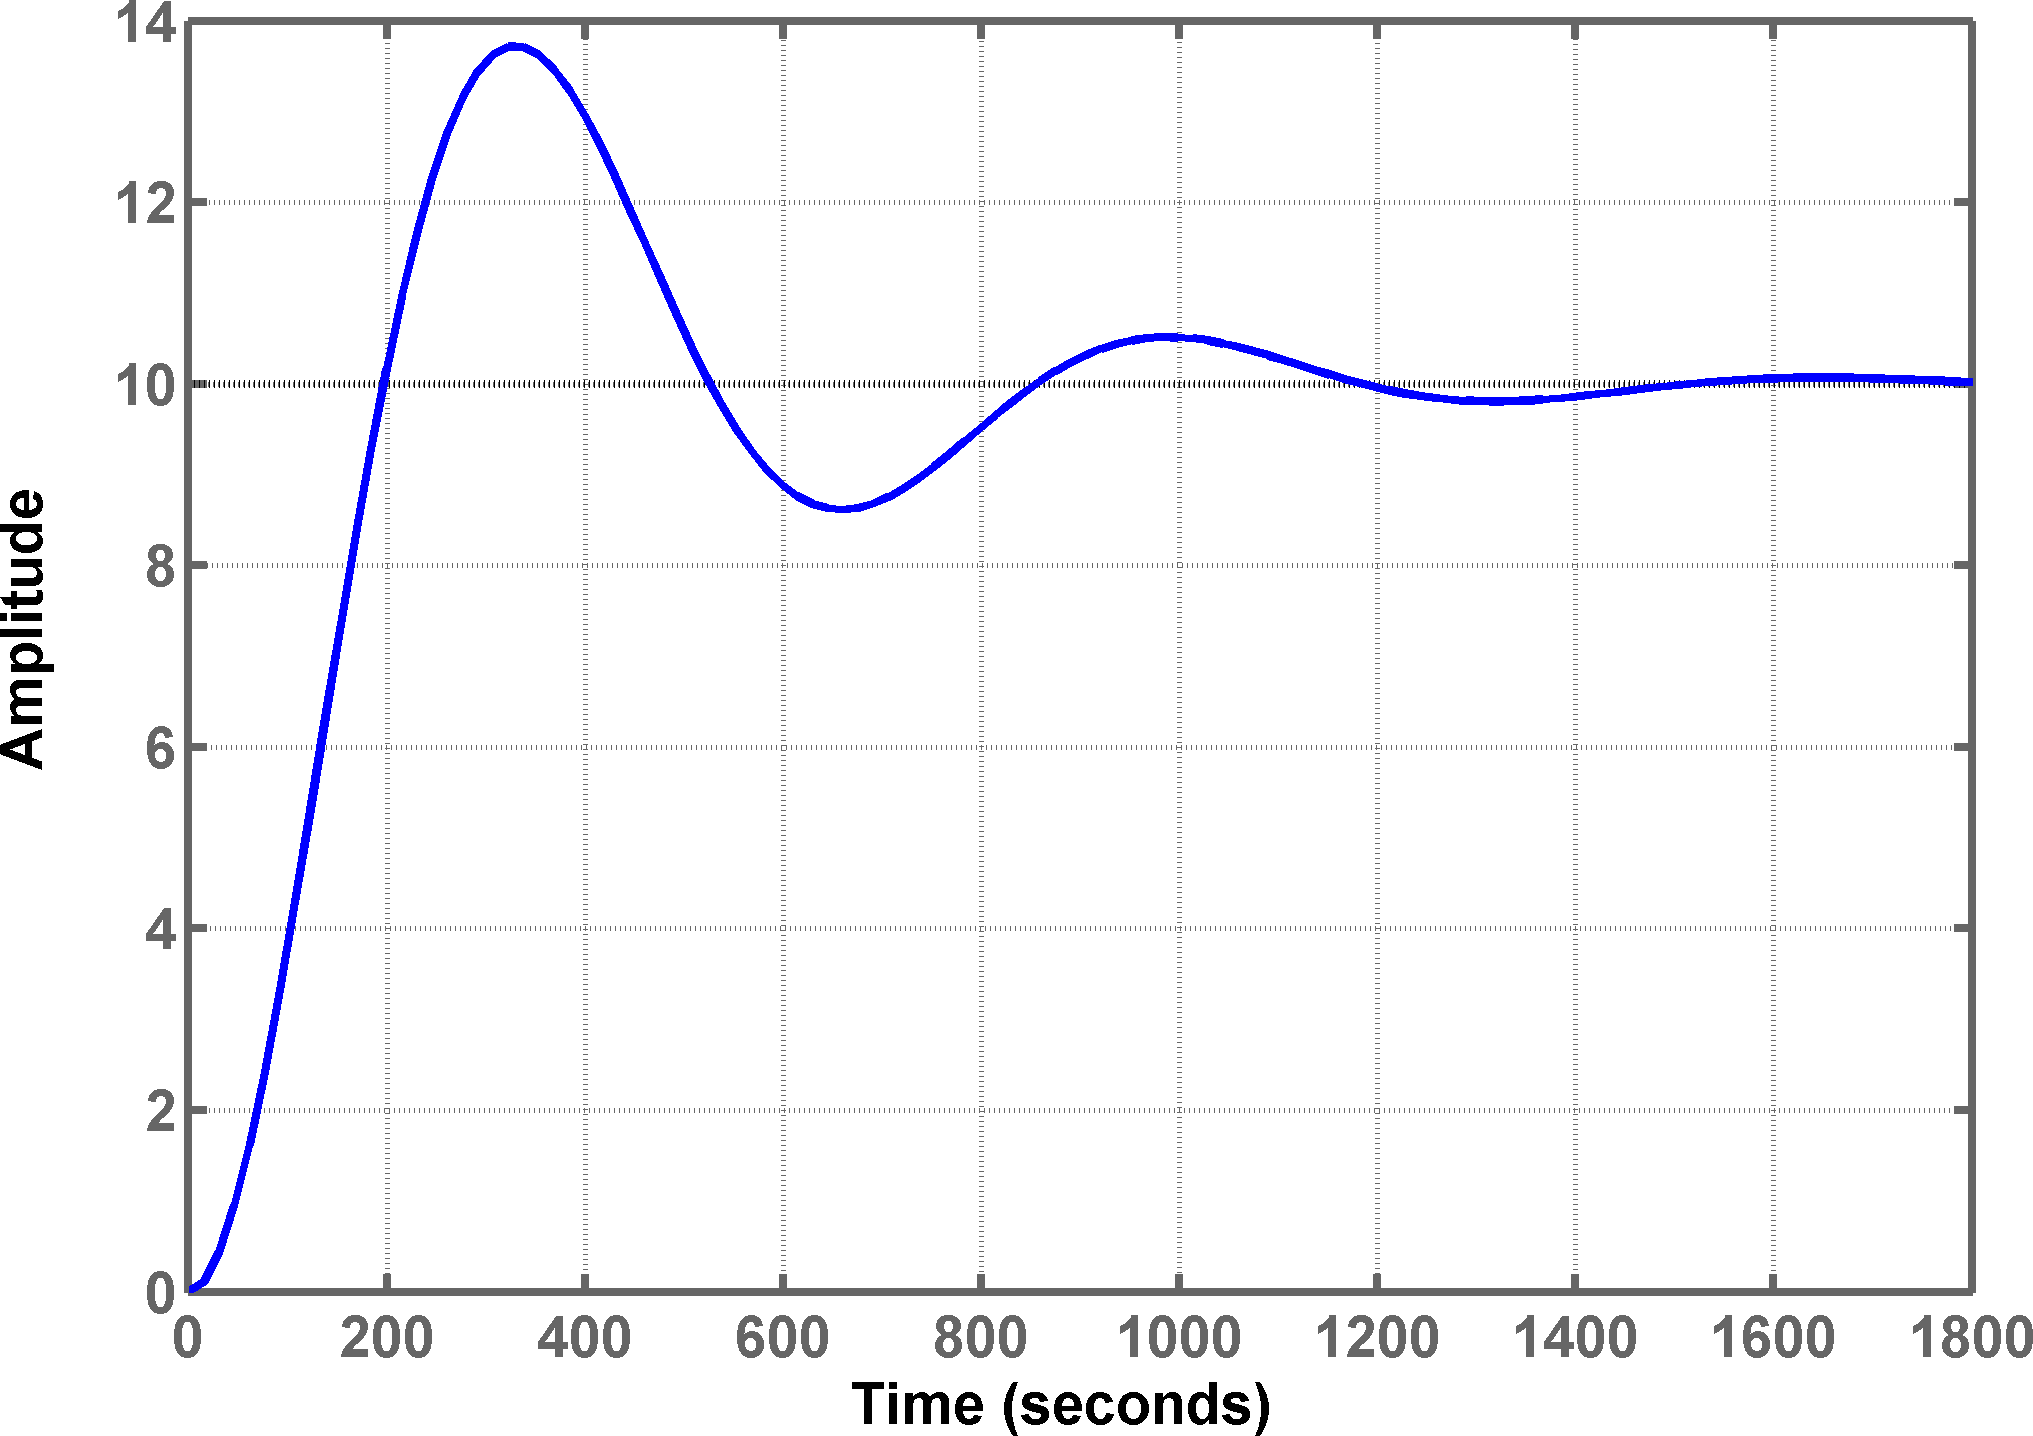
\includegraphics[width=0.6\linewidth]{images/general/step_pt2}
\end{center}
\caption{Step response of a $PT_2$ element}
\label{fig:step_pt2}
\end{figure}

Using the turn tangent principle depicted in Figure \ref{fig:wendetangentenverfahren}, the parameters $T_u$, $T_g$ and $K_s$ were derived.

\begin{figure}[H]
\begin{center}
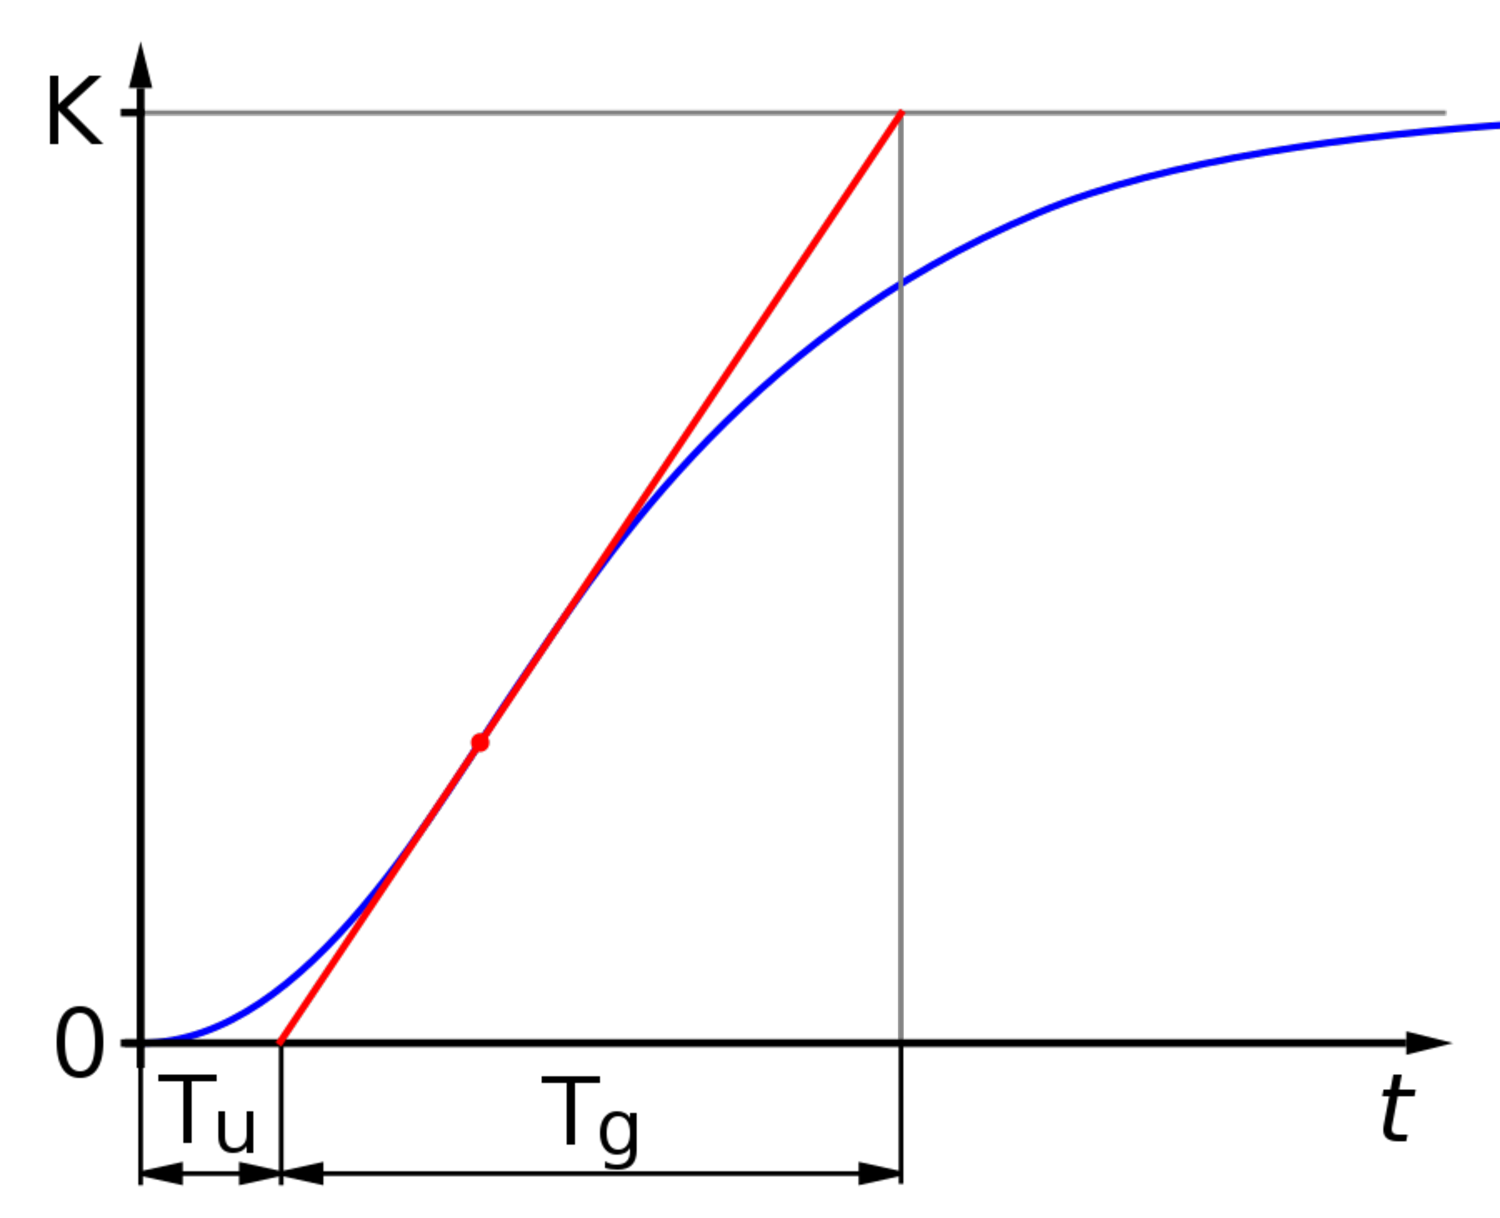
\includegraphics[width=0.6\linewidth]{images/general/wendetangentenverfahren}
\end{center}
\caption{Step response of a $PT_2$ element}
\label{fig:wendetangentenverfahren}
\end{figure}
